\documentclass{article}
\usepackage{amssymb}
\usepackage[utf8]{inputenc}
\usepackage[english]{babel}
\usepackage{amsthm}
\usepackage{enumitem}
\usepackage{amsmath}
\usepackage{mathrsfs}
\usepackage{hyperref}
\usepackage{graphicx}
\usepackage{placeins}
\usepackage[hypcap]{caption}
\usepackage{subcaption}
\usepackage[margin=.5in]{geometry}
\usepackage[export]{adjustbox}
\usepackage{listings}
\usepackage{alltt}

\graphicspath{{../Figures/}}

\title{Project 2 Writeup}
\date{04/20/2016}
\author{Andrea Bajcsy \and Michelle Cody \and Charles Parker }

\begin{document}
	\maketitle
	
	\begin{enumerate}
	
	\item[\textbf{WU1}]
	
	\begin{enumerate}
		\item[(A)] 	 The words most indicative of being Sauvignon-Blanc are ``citrus", ``lime", and ``grapefruit" for OAA and ``citrus", ``"crisp", and ``"lime" for AVA. The words most indicative of not being Sauvignon-Blanc are ``apple" and ``flavors" for OAA and ``enjoy", ``warm", and ``apple" for AVA.
		
		The words most indicative of being Pinot-Noir are ``cherry" for OAA and ``acidity" for AVA. The words most indicative of not being Pinot-Noir are ``cassis" and ``raspberries" for OAA and `cassis" and ``crisp" for AVA.
		
		The words indicative of a particular wine $w$ have the property that when the decision trees branch``Y" on those words, most of the remaining examples are of class $w$. The words in indicative of not being $w$ have the property that when the decision trees branch ``N" on those words, most of the remaining examples are not of class $w$. For example, on the OAA classifier for Sauvignon-Blanc, when the tree branches ``Y" on ``grapefruit", 14 out of the 15 remaining examples are of class Sauvignon-Blanc. So, ``grapefruit" is indicative of class Sauvignon-Blanc.
		
		\item[(B)] The OAA accuracy is 37.29\%. The training time is 0.372 seconds.  The AVA accuracy is 26.15\%.  The training time is 0.387 seconds. The words that suggest Viognier is one of your least favorite wines are ``lovely" and ``enjoy" since the presence of these words indicate that the wine is not Viognier.
		
		\item[(C)] The accuracy for OAA using zero/one predictions is 24.30\%. The accuracy for AVA using zero/one predictions is 26.35\%. The OAA accuracy is much worse than the confidence predictions. Using confidence improves the accuracy by about 50\%. The AVA accuracy is roughly the same for zero/one predictions and confidence predictions. The difference could easily be explained by the random choices made by sklearn.
	\end{enumerate}
	

	\item[\textbf{WU2}] The test accuracy you get with a balanced tree on the WineData using a DecisionTreeClassifier with max depth 3 is 30.89\%.
	
	\item[\textbf{WU3}] 
Negative values of the step size cause the algorithm to diverge (see Figure ~\ref{fig:WU2} for example with step size -5), 0 is constant, and 0.2 converges. We can see in Figure ~\ref{fig:WU2} that 0.5 finds the optimum in one step.
\pagebreak

\begin{figure}[htp]
\centering
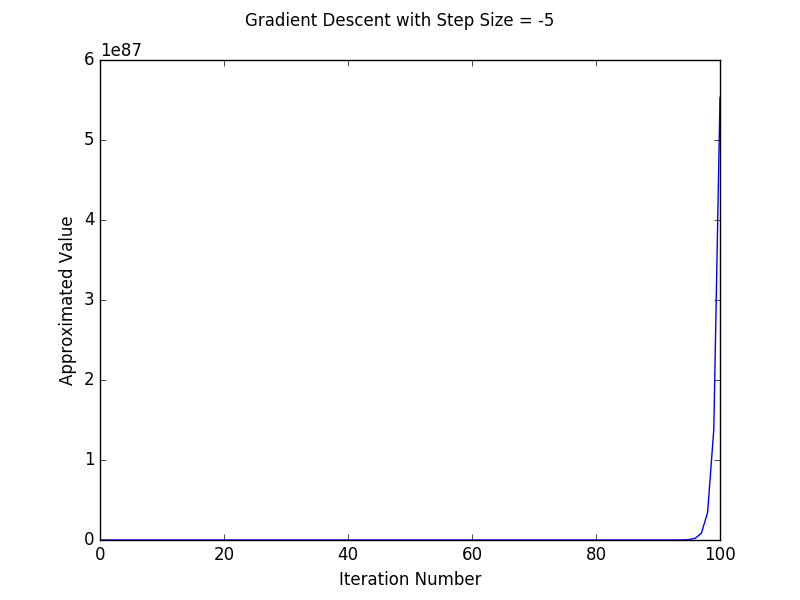
\includegraphics[width=.5\textwidth]{gd_ss_neg5.png}\hfill
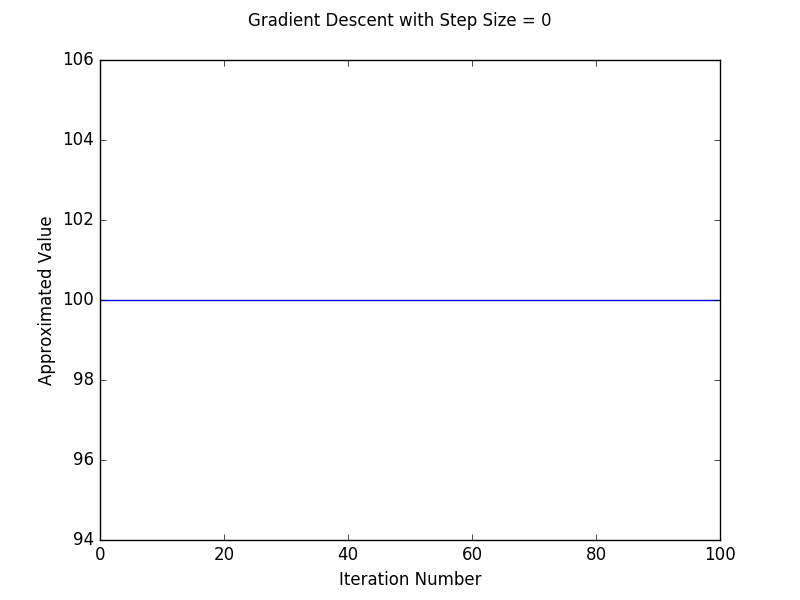
\includegraphics[width=.5\textwidth]{gd_ss_0.png}\hfill
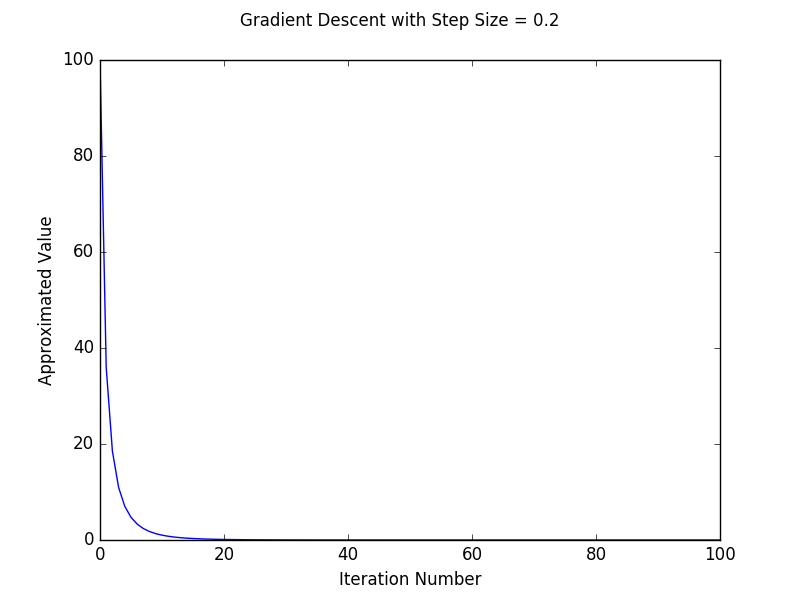
\includegraphics[width=.5\textwidth]{gd_ss_point2.png}\hfill
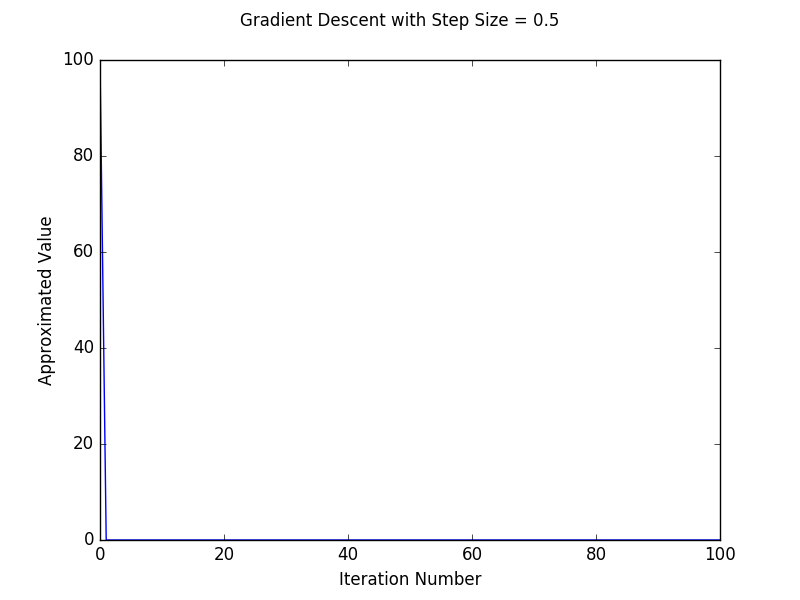
\includegraphics[width=.5\textwidth]{gd_ss_point5.png}
\caption{Gradient Descent performed with 100 iterations with step sizes -5, 0, 0.2, and 0.5.}
\label{fig:WU2}
\end{figure}

	\item[\textbf{WU4}] 
Using the function $x^3+x^{10}-x^2$, we have a non-convex univariate optimization problem with local minima at about (0.606, -0.138) and global minima at (-0.911,-1.192). Looking at Figure ~\ref{fig:WU3}, we see the first run where it gets caught in a local minimum and the second run  where it manages to make it to a global minimum.

\begin{figure}[htp]
\centering
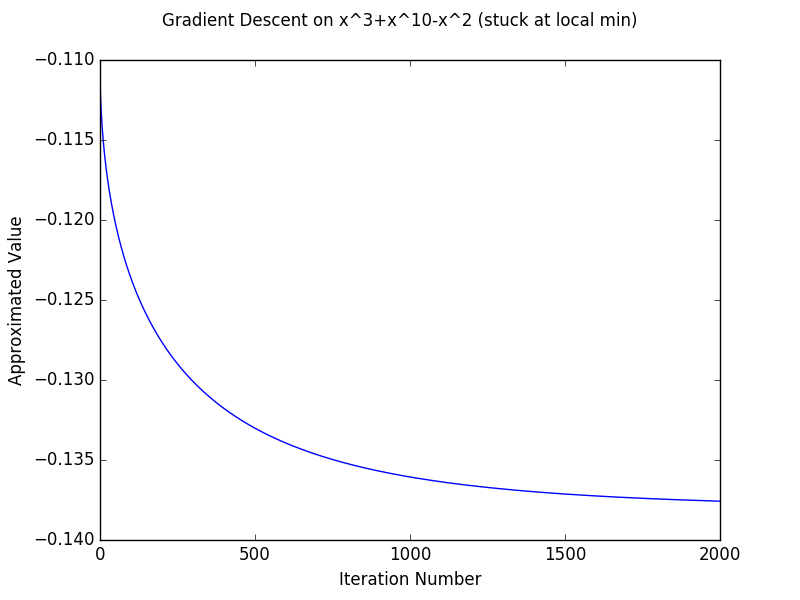
\includegraphics[width=.5\textwidth]{gd_local_min.png}\hfill
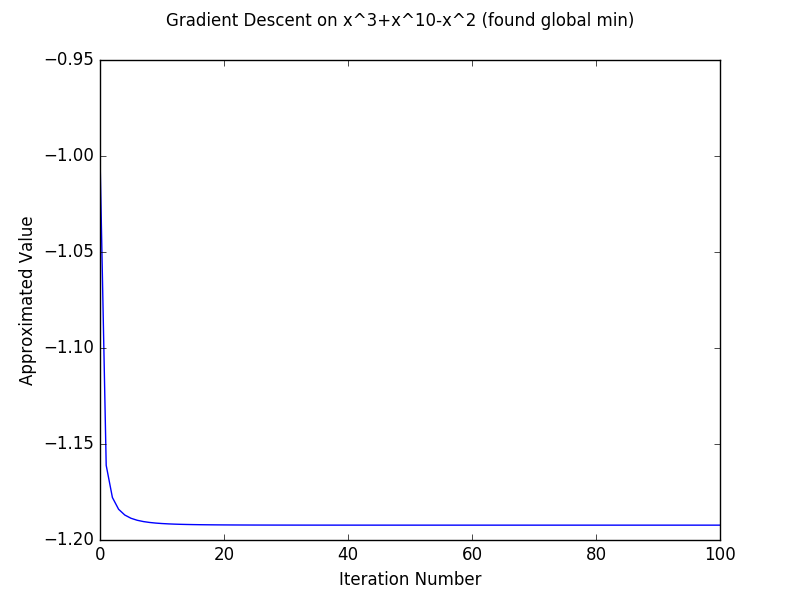
\includegraphics[width=.5\textwidth]{gd_global_min.png}
\caption{Gradient Descent on $x^3+x^{10}-x^2$ that gets trapped at local min (left) or finds global min (right)}
\label{fig:WU3}
\end{figure}

	\item[\textbf{WU5}] 
	
	\begin{enumerate}
		\item[(A)] Squared Loss with \texttt{lambda = 1}, \texttt{numIterations = 8000}, and \texttt{stepSize = .0125}: Training accuracy 0.506073, test accuracy 0.527675
		\item[(B)] Logistic Loss with \texttt{lambda = 1}, \texttt{numIterations = 100}, and \texttt{stepSize = .05}: Training accuracy 0.995951, test accuracy 0.97417
		\item[(C)] Hinge Loss with \texttt{lambda = 1}, \texttt{numIterations = 100}, and \texttt{stepSize = .05}: Training accuracy 0.753036, test accuracy 0.686347 
		
	\end{enumerate}
	
	The logistic loss function produced the best results, as shown above. The words corresponding to the weights with the greatest negative value are ``tannis", ``black", ``dark", ``cherry", and ``blackberry". The association with high negative weights means that these words are more indicative of class -1 than any other words. The words corresponding to the weights with the greatest positive values are ``citrus", ``crisp", ``lime", ``acidity", and ``tropical". The association with high positive weights means that these words are more indicative of class 1 than any other words. This group of words is the best group to make predictions. In this context, ``best" means that using only these words as features, one would expect the highest accuracy over using any other group of words. The results for the positive words agree with the words indicative of Sauvignon-Blanc from \textbf{WU1}.
	
	\end{enumerate}

\end{document}

